\section{Experimental methods}\label{supp:fields}\label{supp:metrics}
\subsection{Network, path sets, and demand settings}\label{supp:networks}
The public Sioux Falls network has $24$ nodes and $76$ directed arcs
\citep{tnfrc2024transportation}. All arcs belong to one block atom, hence
one compatibility class. The eight queries are the positive-demand OD pairs with the largest
published demands, with ties broken by ascending origin then destination
node ID. All happen to involve node $10$.
The queries are
$(10,16)$, $(16,10)$, $(10,11)$, $(10,15)$, $(15,10)$, $(10,17)$, $(11,10)$, $(17,10)$,
with published demands
$q_{\mathrm{base}}=(4400,4400,4000,4000,4000,3900,3900,3900)$ veh/h.
The attribution path changes these demands from $0.2q_{\mathrm{base}}$ to
$1.6q_{\mathrm{base}}$. Node IDs in the traffic experiments are one-based.
Flows retain the benchmark's approximate-hourly convention; one time unit
is $0.01$ h. A reported TSTT number is $\sum_e F_et_e(F_e)$ with $F_e$
in veh/h and $t_e$ in these time units: multiplying by $0.01$ gives the
hourly vehicle-hour total, without extrapolating to a day. All absolute
attribution and boundary-account numbers use the same convention.

For each OD we retain every loopless directed path if enumeration finishes
within $200$ paths, otherwise the ten shortest by free-flow cost (Yen's
algorithm, lexicographic edge-sequence tie breaking); no OD in this
network has a fully enumerated set under the threshold. All eight query
ODs use ten paths. The link--path incidence $\Delta$ and the matrix $A$
summing paths within each OD stay fixed, so $B\Delta=MA$ with the
appropriate full or study OD incidence matrix. The full-background
ten-path set has $5{,}280$ paths (ten per OD; the expanded set
$10{,}560$, twenty per OD); Appendix~\ref{supp:coverage} compares these
candidate-path models.

The path-exchange response space $T_{\mathrm{swap}}=\Delta\ker A$
(Appendix~\ref{app:membership}) has dimension $32$ in A with ten
paths for each study OD, and dimension $53$ in C with either ten or
twenty paths for every OD, equal to the full circulation-space
dimension $m-n+1=53$ (ranks computed from within-OD differences of
link--path incidence columns, cross-checked against singular-value
bases of $\Delta\ker A_{\mathrm{OD}}$). On Sioux Falls, full background
therefore spans the complete circulation space through allowable path
exchanges, while the eight-OD path model spans a proper subspace. On Anaheim, whose
centroid-restricted ten-path sets cannot use nodes $2$--$38$ in
transit, $T_{\mathrm{swap}}$ has dimension $404$ of a circulation-space
dimension of $499$: a proper subspace, although still large enough
that the model-specific weight tests fail decisively there
($\rho_{\mathrm{swap}}=2.2$).

The three demand settings share the same query endpoints. In the
no-background setting, all other demands are zero. In the
frozen-background setting, assign all positive
background demands jointly with the study demands fixed at
$q^0=0.2q_{\mathrm{base}}=(880,880,800,800,800,780,780,780)$ veh/h in
the listed query order, freeze the resulting background link flows, and
re-equilibrate only the eight query ODs. In the responsive-background assignment, the other $520$
positive OD demands stay at published values while all $528$ ODs
re-equilibrate jointly at every path point and perturbation. TSTT and
its gradient use total link flows in the frozen- and responsive-background assignments; the latter is a
full-background assignment with eight attribution queries, not an
attribution evaluation of all $528$ ODs.

\subsection{Equilibrium and its sensitivities}\label{supp:sue}
Unless stated otherwise, the fixed-path logit stochastic user equilibrium
(SUE) uses $\theta=1$ and BPR costs
$t_e(F_e)=t_{0,e}[1+0.15(F_e/c_e)^4]$. With $\Pi_j$ the path set,
\begin{equation}
h_p=q_jp_p(F),\quad
p_p(F)=\frac{\exp[-\theta(\Delta^\top t(F))_p]}
{\sum_{r\in\Pi_j}\exp[-\theta(\Delta^\top t(F))_r]},\quad
F=\Delta h.\label{eq:sueloading}
\end{equation}
This is the solution of
\[
\min_{h\ge0,\ Ah=q}\left\{
\sum_e\int_0^{(\Delta h)_e}t_e(s)ds+
\theta^{-1}\sum_p h_p(\log h_p-1)\right\}.
\]
For positive demands the feasible set is nonempty and compact, the
objective strictly convex, and the minimizer positive: transferring
mass to a zero path flow from a positive path of the same OD improves
the objective, with entropy change
$\theta^{-1}\epsilon\log\epsilon+O(\epsilon)<0$. Its Hessian and
sensitivity equations are
\begin{equation}
H=\Delta^\top\operatorname{diag}(t'_e)\Delta+
\theta^{-1}\operatorname{diag}(1/h_p)\succ0,\qquad
\begin{bmatrix}H&A^\top\\A&0\end{bmatrix}
\begin{bmatrix}\partial_jh\\\partial_j\nu\end{bmatrix}
=\begin{bmatrix}0\\\mathbf e_j\end{bmatrix}.
\label{eq:kkt_sensitivity}
\end{equation}
$A$ has full row rank, so the system is nonsingular and the implicit
function theorem gives a $C^1$ demand-to-flow map.

For the responsive-background assignment we solve the equivalent total-link-flow fixed
point $F=L(F,q)=\Delta\{q_jp_{\Pi_j}(F)\}_j$ by Newton steps with residual
line search. For the frozen-background setting the corresponding equation is
$F=F_{\mathrm{bg}}^0+\Delta_{\mathrm{study}}
\{q_jp_{\Pi_j}(F)\}_{j\in\mathrm{study}}$, where $F_{\mathrm{bg}}^0$
is fixed at the joint $q^0$ equilibrium. Costs and gradients use this
total $F$ in both equations. Every solution is checked against its path-loading
equation, with maximum absolute path-flow gap below $10^{-7}$ veh/h.
The $76$-dimensional implicit system avoids forming a dense path Hessian.
For an OD group $R$, define
\[
S_R=\theta\sum_{k\in R}\Delta_k
\left[\operatorname{diag}(h_k)-h_kh_k^\top/q_k\right]\Delta_k^\top,
\quad W=\operatorname{diag}(t'_e(F_e)),\quad S=S_{\mathrm{all}}.
\]
Differentiating the logit probabilities gives
$\partial_F L_R=-S_RW$. Consequently the total sensitivity satisfies
\begin{equation}
(I+SW)J_j=\Delta_jp_j,\qquad
J_j^{\mathrm{study}}=\Delta_jp_j-S_{\mathrm{study}}WJ_j,\qquad
J_j^{\mathrm{bg}}=-S_{\mathrm{bg}}WJ_j.
\label{eq:bg_sensitivity}
\end{equation}
Here ``study'' includes all eight queried ODs and ``background'' the
other $520$: $J_j=J_j^{\mathrm{study}}+J_j^{\mathrm{bg}}$,
$BJ_j^{\mathrm{study}}=\mu_j$, $BJ_j^{\mathrm{bg}}=0$, the study
term including responses of the other seven study ODs. The
decomposition uses one joint equilibrium, rather than sensitivities
at different congestion states.
In the frozen-background setting the background flows have no
derivative, so the same
implicit system uses $S=S_{\mathrm{study}}$, with
$J_j^{\mathrm{study}}=J_j$ and $J_j^{\mathrm{bg}}=0$.

Central finite differences independently re-solve Eq.~\eqref{eq:sueloading}
at $q\pm a_j\mathbf e_j$, $a_j=0.005q_{\mathrm{base},j}$ and
$a_j/2$; both steps are checked at every $\theta=1$ ten-path
responsive-background integration point, the path-set and $\theta$ variations
add half-step checks for all eight columns at the path midpoint, and
the link Newton solver is compared against the successive-averages
background equilibria at their common eleven quadrature points.

\subsection{Conservative learned surrogate}\label{supp:protocol}
The zero-background surrogate parameterizes
$h_j=q_j\operatorname{softmax}(z(q)|_{\Pi_j})$, $f=\Delta h$.
The three hidden layers each have $128$ tanh units; the final layer is
linear. The logit head uses training-standardized demands while the raw
$q_j$ multiplies the shares, preserving nonnegative flow and exact
conservation. Computations use double precision.
Training targets are fixed-path logit-SUE assignments ($\theta=1$,
path fixed-point tolerance $10^{-6}$). The $2500/857/857$
training/validation/test split uses seed $20260820$, with demands
$q_j=q_{\mathrm{base},j}s_j$ and independent $s_j$ drawn from
LogNormal$(0,0.5^2)$ clipped to $[0.2,2]$.
Adam uses learning rate $0.003$, full-batch link-flow MSE, at most
$12{,}000$ steps, and validation every $50$ steps. The
minimum-validation-error state of each seed $0,\ldots,4$ supplies
the reported results, with automatic differentiation supplying their
Jacobians; the test split is used only for final reporting.

\subsection{Integration grids, connected boundaries, and cancellation diagnostics}\label{supp:quadrature}
All numerical integrations use composite trapezoids. The principal
learned zero-background results use $201$ quadrature points; direct
zero-background SUE and both background settings use $41$ in the main
table. The frozen-background setting compares $11$ with $41$ points;
the responsive-background setting
compares $11$, $21$, and $41$ nested points; the two near-balanced
queries add $81$ and $161$ nested points; the learned-versus-SUE
sensitivity comparison uses identical $41$-point grids, kept separate
from the $201$-point learned results (Appendix~\ref{supp:accuracy}).

Connected boundaries require both $G[U]$ and $G[V\setminus U]$ to be
connected on the underlying undirected graph, with $s_j\in U$, $t_j\notin U$.
Exact enumeration yields $10{,}270$--$13{,}253$ admissible sets for each
of the eight main study ODs, and $4{,}621$--$16{,}943$ for the six
additional queries of Appendix~\ref{supp:newod}.
Extrema of $-\mathbf1_U^\top B\widetilde C_j$ are evaluated by exact
enumeration, cross-checked against independent subset enumeration on
restricted neighborhoods; attaining sets are verified for membership
with values recomputed by direct summation.

For cancellation diagnostics define
$A_j=|\Delta q_j|\int_0^1\sum_{v\notin\{s_j,t_j\}}|(BD_\lambda J_j)_v|d\lambda$
and $\kappa_j=1-S_j/A_j$ when $A_j>0$. The triangle inequality gives
$0\le S_j\le A_j$. Both quantities use the specified $201$-point learned
grid and are summarized over the five seeds; checks on additional
path-set or dispersion models sample the demand-path midpoint and
endpoints.

\subsection{Six pre-specified queries away from node 10}\label{supp:newod}
The selection rule uses only published demands and free-flow
shortest-path times. Candidates are the positive-demand ODs whose origin
and destination both differ from node $10$; ranking them by demand and
splitting into three equal-count terciles, the minimum- and
maximum-free-flow-shortest-path OD within each tercile is selected, with
ties broken by ascending (origin, destination). The six queries are
$(7,18)$, $(1,19)$, $(4,5)$, $(1,15)$, $(6,8)$, and $(7,12)$, with
published demands $(200,300,500,500,800,700)$ veh/h and free-flow
shortest-path times $(2,22,2,23,2,19)$ time units; the joint
protocol, sensitivities, and boundary enumeration are as in
Section~\ref{subsec:newod}, with conservation checks at responsive-background
floating-point levels (maximum path fixed-point residual
$1.6\times10^{-10}$ veh/h, midpoint implicit-versus-finite-difference
column error $2.6\times10^{-8}$, completeness $4.3\times10^{-7}$).

For the single-OD checks, let $\bar q=q^{\mathrm{base}}$ be the full
published demand vector over all $528$ positive-demand ODs. For each
focal query $j\in\{(1,19),(1,15),(7,12),(6,8)\}$, define
\begin{equation}
q^{(a)}=\bar q+(a q_j^{\mathrm{base}}-\bar q_j)e_j,
\qquad
q^{(b)}=\bar q+(b q_j^{\mathrm{base}}-\bar q_j)e_j,
\qquad
(a,b)\in\{(0.2,1.6),(0.9,1.1),(0.8,1.2)\},
\label{eq:singleodstates}
\end{equation}
where $e_j$ is the coordinate unit vector. All other $527$ demands,
including the other five selected queries, remain at their published
values $\bar q_{-j}$ along the segment. Direct equilibria and the learned
small-band checks use these same reference states. The responsive-background solver,
path sets, and boundary definitions are unchanged; checks and interval
results are in Appendix~\ref{supp:newodaccuracy}. For each interval,
Eq.~\eqref{eq:edgeidentity} gives the attribution column from the two
endpoint equilibria alone.

\subsection{Same-task computation timings}\label{supp:timing}
All timings describe the same fixed tasks and the same computational
environment that produced the reported accounts
(Section~\ref{sec:stability}). For the separable single-OD task on
query $(1,19)$ (only its demand changes, with endogenous rerouting;
shared path set, solver tolerance and $152$-region family; medians of
three uncached runs), the endpoint identity computes the attribution
column in $0.088$ s against $0.510$, $0.948$ and $1.813$ s for $21$-,
$41$- and $81$-state sensitivity integration, whose account columns
agree with the endpoint values to $6.6\times10^{-5}$,
$1.6\times10^{-5}$ and $4.1\times10^{-6}$ in maximum absolute
geometric-account error; the identity eliminates sensitivity
integration for separable single-OD tasks but does not separate OD
columns when several demands change jointly. For spatial aggregation
of a fixed region family once reference columns are available, the
three methods of Section~\ref{sec:scan} agree to
$2.2\times10^{-11}$ TSTT units on the $1{,}642$ oriented Sioux Falls
regions: the prefix scan takes $4.16$ ms per six columns
($87.92$ ms per 120), the vectorized one-sparse-product
$A_{\mathcal F}C$ takes $0.24$ ms per six ($3.46$ ms per 120) after a
one-time $69.5$ ms matrix build, and direct crossing-edge summation is
slowest ($28.51$/$1{,}176.15$ ms); on the $910$ Anaheim query--region
accounts the same ordering holds ($0.10$/$0.30$/$13.31$ ms), with
agreement to $5.9\times10^{-12}$ against node sums, and the $21$-state
reference construction, including paths and sensitivities, took
$1{,}278.7$ s.

\subsection{Anaheim network, equilibrium and predefined regions}\label{app:anaheimsettings}
Both network and demand files are the public Transportation Networks for Research Core Team Anaheim TNTP data \citep{tnfrc2024transportation}. The network header supplies free-flow times in minutes and capacities in vehicles per hour; all roads use the published BPR coefficient 0.15 and power 4. We use $t_e(F_e)=t_e^0[1+0.15(F_e/c_e)^4]$ and TSTT marginal weight $t_e^0[1+0.75(F_e/c_e)^4]$. The six study OD demands, ranked by descending base demand and then lexicographic OD, are $(4,2)$: 2106.7, $(1,2)$: 1365.9, $(2,4)$: 1271.4, $(3,2)$: 1237.9, $(25,4)$: 1232.4, $(25,2)$: 1232.3 vehicles per hour. They move jointly from 0.8 to 1.2 times base demand; all remaining positive demands stay at their published base values and retain endogenous route choice. Every OD uses ten loopless free-flow shortest routes from Yen's algorithm. Ties within $10^{-12}$ minutes are resolved by lexicographic edge-index sequence in the TNTP road order. Nodes 1--38 are centroids and cannot be intermediate route nodes; the first through node is 39. Logit scale $\theta=1$ minute$^{-1}$ applies to route travel time in minutes.
The edge Newton solver targets maximum loading residual below $10^{-8}$ vehicles per hour, uses at most 80 iterations and backtracking up to 30 halvings per step, and checks the original path loading residual below $10^{-7}$. Implicit derivatives solve the same fixed-point equation. Trapezoidal integration uses equally spaced states, with warm starts from a neighboring saved state. The 41-state refinement reuses all 21 old states and computes only the twenty new midpoints.
The distance-based region construction and fixed progress targets are specified in Section~\ref{sec:anaheim}. The reported range uses every admissible prefix in that family. Same-state mechanisms compare regions chosen nearest the progress targets, using free-flow weights $t^0$ and congestion weights equal to the total-flow TSTT marginal weight minus $t^0$. Figure~\ref{fig:anaheimrest} plots the five profiles not shown in the main text.
\begin{figure}[pos=htbp]\centering
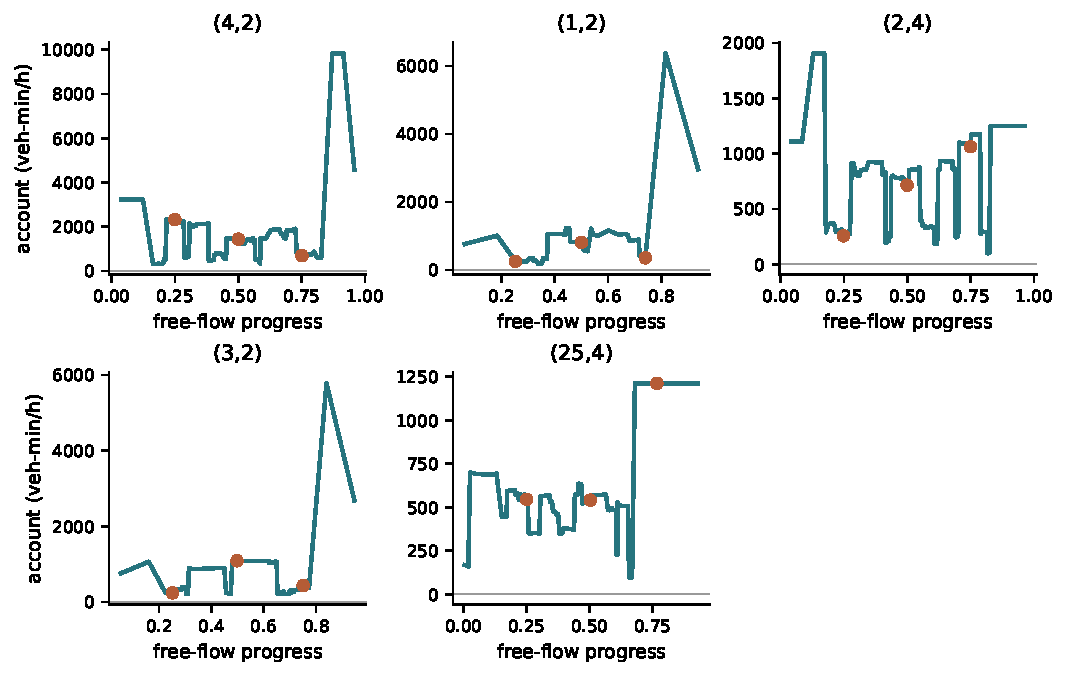
\includegraphics[width=0.99\linewidth]{../figures/fig_v108_anaheim_rest.pdf}
\caption{Anaheim spatial response profiles of the remaining five study
queries over the distance-based families: the account versus free-flow
progress along each query's own OD direction, with ochre dots marking
the three prespecified positions. All stay positive; family ranges span
roughly one to one and a half orders of magnitude.}\label{fig:anaheimrest}
\end{figure}
\begin{table}[pos=htbp]\centering\footnotesize\caption{Anaheim accounts over the complete distance-based family, with the three prespecified positions (vehicle-minutes per hour). Column heads are the prespecified targets; the exact selected levels are (row order) $0.250/0.501/0.752$, $0.252/0.500/0.740$, $0.248/0.499/0.750$, $0.251/0.498/0.751$, $0.251/0.504/0.768$ and $0.250/0.500/0.724$.}\label{tab:anaheim}\begin{tabular}{lrrrrrrr}\toprule OD & System & Unrestricted range & Family range & Regions & $\phi(0.25)$ & $\phi(0.50)$ & $\phi(0.75)$\\\midrule
(4,2) & 34664.1 & [-12712.6,20514.0] & [307.5,9832.1] & 211 & 2323.5 & 1441.8 & 692.3\\
(1,2) & 16773.6 & [-6032.2,9762.0] & [172.7,6374.8] & 83 & 259.0 & 818.0 & 360.5\\
(2,4) & 12143.7 & [-4374.6,6733.0] & [98.7,1905.9] & 211 & 257.0 & 714.6 & 1061.8\\
(3,2) & 14706.7 & [-5613.8,9052.9] & [202.8,5777.4] & 157 & 236.2 & 1087.3 & 434.6\\
(25,4) & 6919.3 & [-1805.3,3091.8] & [96.8,1212.2] & 164 & 545.6 & 540.7 & 1212.2\\
(25,2) & 11445.9 & [-4157.3,6904.5] & [131.8,5751.2] & 84 & 801.5 & 412.0 & 5751.2\\
\bottomrule\end{tabular}\end{table}
\begin{table}[pos=htbp]\centering\footnotesize\caption{Anaheim differences between preselected early and late regions, split by free-flow and congestion weights and study and background responses (vehicle-minutes per hour).}\label{tab:anaheimmechanism}\begin{tabular}{lrrrrr}\toprule OD & Free-flow study & Free-flow background & Congestion study & Congestion background & Total\\\midrule
(4,2) & -416.91 & -8.53 & -1499.94 & 294.16 & -1631.21\\
(1,2) & 9.85 & 6.96 & 83.01 & 1.71 & 101.54\\
(2,4) & 312.07 & -65.41 & 667.06 & -108.90 & 804.83\\
(3,2) & 50.04 & 11.80 & 136.55 & 0.04 & 198.43\\
(25,4) & 47.28 & -40.11 & 666.28 & -6.89 & 666.56\\
(25,2) & -131.77 & -10.52 & 5102.23 & -10.15 & 4949.79\\
\bottomrule\end{tabular}\end{table}

\subsection{Learning objectives and exact endpoint targets}\label{app:learning-objectives}
Equation~\eqref{eq:localboundarybound} suggests learning the reference's weighted demand response
where it affects spatial accounts. With training-only positive scales
$a_j$, the boundary term is
\begin{equation}
\mathcal L=\mathcal L_{\mathrm{flow}}+\lambda_J\mathcal L_{\mathrm{response}}
+\lambda_{\mathrm{cut}}\mathcal L_{\mathrm{boundary}},\qquad
\mathcal L_{\mathrm{boundary}}
=\frac1{NK}\sum_{q,j}\left[\frac{\mathcal K_j(h_j(q))}{a_j}\right]^2.
\label{eq:trainingobjective}
\end{equation}
The reference Jacobian is obtained from the existing implicit SUE
sensitivity system (Appendix~\ref{supp:sue}). The empirical study
compares six objectives under a shared continuation protocol
(Appendix~\ref{app:pairs-v102}): flow only; the unweighted response
$\|J_j^L-J_j^S\|$; the weighted response $\|D^LJ_j^L-D^SJ_j^S\|$ of
Eq.~\eqref{eq:coldecompmain}; the pointwise boundary seminorm
$\mathcal K_j(D^LJ_j^L-D^SJ_j^S)$ of Eq.~\eqref{eq:trainingobjective};
and the two endpoint objectives below.
Derivative supervision itself is established in Sobolev training
\citep{czarnecki2017sobolev}, including finite-difference derivative targets
\citep{yuan2022sobolev}; the network-derived target here selects the
part of weighted response error that changes boundary accounts.
A circulation in $\ker B$ is invisible to $\mathcal K_j$, so flow and
response losses remain necessary for the other attribution objectives.
The target matches the reference's actual response; it does not force
its true internal attribution divergence to zero or replace TSTT weights
with uniform weights. Equation~\eqref{eq:localboundarybound} is a path
inequality; finite training-point losses alone do not certify an entire
demand domain.


For the following finite-change statement, the outcome is explicitly separable:
\[
g(F)=(g_e(F_e))_{e\in E},\qquad T(F)=\sum_{e\in E}g_e(F_e).
\]
\begin{proposition}[exact finite-change boundary target]\label{prop:pairboundary}
Let $f^L,f^S$ and the edgewise outcome $g$ be continuously differentiable
on an open demand domain, and let $q^\pm=q\pm h e_j$ with their entire
segment in that domain. Put
\[
z_j^r=g(f^r(q^+))-g(f^r(q^-)),\qquad r\in\{L,S\}.
\]
For the attribution of this single-OD change,
\begin{equation}
\max_{U:s_j\in U,\ t_j\notin U}|\phi_j^L(U)-\phi_j^S(U)|
=\mathcal K_j(z_j^L-z_j^S).\label{eq:pairboundaryexact}
\end{equation}
If all sufficiently small single-coordinate changes have matching
accounts on every separating boundary at every point of the domain,
then $BD^LJ_j^L=BD^SJ_j^S$ throughout the domain. Integrating yields
matching boundary attribution columns for any joint demand path in that
domain (with the same columnwise path convention).
\end{proposition}
Appendix~\ref{app:pairproof} proves both statements. The first is an
exact finite-change target, whereas the pointwise response objective
optimizes the upper bound in Eq.~\eqref{eq:localboundarybound}; integrating
before taking $\mathcal K_j$ can retain cancellations. The second statement
requires a domain-wide local premise and is not a guarantee from finite
training data. With several ODs changing, the endpoint outcome difference
only identifies the sum of their attribution columns.

For sampled single-OD endpoint pairs, a direct training objective is
\begin{equation}
\mathcal L_{\mathrm{pair}}=\mathcal L_{\mathrm{flow}}
+\lambda_{\mathrm{edge}}\frac1N\sum_{(q,h,j)}
\frac{\|z_j^L-z_j^S\|_2^2}{b_j^2}
+\lambda_{\mathrm{cut}}\frac1N\sum_{(q,h,j)}
\left[\frac{\mathcal K_j(z_j^L-z_j^S)}{a_j}\right]^2,
\label{eq:pairobjective}
\end{equation}
with positive training-only scales $a_j,b_j$. The edge term controls
changes invisible to the boundary seminorm, whose kernel is $\ker B$.
Two reference endpoint equilibria supply $z_j^S$; training uses ordinary
parameter backpropagation through two predictions, without reference
Jacobian labels or input-Jacobian differentiation.

\subsection{Learned-model evaluation protocol}\label{app:pairs-v102}
Six objectives continue each of five common conservative models for
1,200 Adam updates, with learning rate $3\times10^{-5}$, flow batch 32
and query batch eight. The flow data and seed-specific minibatch
sequences are shared. Each of six queries has 64 training and 16
validation endpoint pairs. Centers are sampled coordinatewise from
$[0.65,1.3]$ times baseline demand (seed 102111); half-widths 2.5\% and
15\% occur equally often. Only one demand changes per pair, while
background routes remain responsive.

The flow loss averages $[(f_e^L-F_e^S)/s_e]^2$ over minibatch states
and edges, with $s_e=0.01\sqrt{\operatorname{mean}_{\rm train}[(F_e^S)^2]}$ from the
2,500 training states. Each auxiliary objective adds one term
$\lambda\,\mathcal L_{\mathrm{aux}}$ to this flow loss, with the weight
grid $\lambda\in\{0.001,0.003,0.01,0.03,0.1,0.3,1\}$ searched
identically for every objective. Each normalizer carries the units of
its own target, so that the common grid explores comparable
regularization ranges: rescaling the outcome $T\mapsto cT$ rescales
the weighted terms' normalizers with them and leaves every effective
weight unchanged. With
$\langle\cdot\rangle_j$ denoting the average over query $j$'s training
centers or endpoint labels, the training-only scales are
\[
\begin{aligned}
u_j&=\max\{\sqrt{\langle\|J_j^S\|_2^2\rangle_j},10^{-6}\},&
v_j&=\max\{\sqrt{\langle\|D^SJ_j^S\|_2^2\rangle_j},10^{-6}\},&
b_j&=\max\{\sqrt{\langle\|z_j^S\|_2^2\rangle_j},10^{-6}\},\\
a_j&=\max\{\sqrt{\langle\mathcal K_j(z_j^S)^2\rangle_j},10^{-6}\},&
\bar a_j&=\max\{\sqrt{\langle\mathcal K_j(D^SJ_j^S)^2\rangle_j},10^{-6}\}.
\end{aligned}
\]
The auxiliary terms are: unweighted response
$\langle\|J_j^L-J_j^S\|_2^2/u_j^2\rangle$; weighted response
$\langle\|D^LJ_j^L-D^SJ_j^S\|_2^2/v_j^2\rangle$, with
$D^r=\operatorname{diag}(\nabla T(F^r))$ the outcome-gradient weights
of Eq.~\eqref{eq:Cdef} evaluated at each model's own flows (TSTT:
$\nabla_eT=t_e+F_et'_e(F_e)=t_{0,e}[1+0.75(F_e/c_e)^4]$);
the pointwise boundary seminorm
$\langle[\mathcal K_j(D^LJ_j^L-D^SJ_j^S)/\bar a_j]^2\rangle$; the
endpoint-edge term
$\langle\|z_j^L-z_j^S\|_2^2/b_j^2\rangle$; and the endpoint-cut bundle,
which adds $0.01$ times
$\langle[\mathcal K_j(z_j^L-z_j^S)/a_j]^2\rangle$ to the endpoint-edge
term (a fixed-ratio ablation of the earlier protocol's internal
mixture, not an independently tuned objective). The three
response-family objectives share one set of derivative labels; the two
endpoint objectives share one set of endpoint labels. The weighted
objective was rerun under this own-scale normalization at every grid
weight from the frozen initializations; under the shared-scale
normalization used in an earlier draft its effective weights were
$v_j^2/u_j^2\approx5$--$1568$ times larger, which is why only the
smallest grid values trained there.

Checkpoint selection uses one uniform rule for every objective and
weight: among the common initial model (update zero) and every 100th
continuation update whose validation flow error is at most $1.1$ times
the initial model's value, take the minimum validation boundary
mean-square error, using the same 96 validation pairs throughout. The
initial model ensures the pool is never empty. The weight $\lambda^*$ of
each objective is then chosen on validation data only: among the grid
values whose seed-median selected validation flow error stays within
$1.1$ times the seed-median initial error, minimize the seed-median
validation boundary error. The flow-only control reuses the frozen
flow continuation under the same uniform rule. Test paths never enter
selection or weight choice. The extended-budget replication of
Section~\ref{sec:pairresults} repeats the response and flow
continuations with 3{,}600 updates under this unchanged protocol
(prefix verified against the archived runs; per-network costs in
Appendix~\ref{app:anaheimlearning}).

The final evaluation uses 96 fixed test paths, all generated by one
rule: for each active-query group $k\in\{1,2,3,6\}$, draw a base state
uniformly from $[0.65,1.3]$ times baseline demand, choose the $k$
active queries in round-robin order, add independent changes of
$15$--$30\%$ of their baseline demands with alternating same-direction
and mixed-direction signs, and solve all 41 states of the resulting
straight demand path. Twenty-four paths (six per group, seed 102112)
and seventy-two paths (eighteen per group, seed 102113) were generated;
models and validation choices were frozen before evaluation on the
additional paths. For every path, flow error first averages relative
Euclidean errors across its states. Attribution statistics average active
queries and seeds within each path and then take medians across the 96 paths;
seeds do not add independent paths. For column error $e_j$ and reference column
$c_j$, relative column, system and unrestricted-boundary errors divide
$\|e_j\|_2$, $|\mathbf1^\top e_j|$ and $\mathcal K_j(e_j)$ by the
corresponding reference values, with absolute floor $10^{-6}$. Geometric error
uses $\max_{U\in\mathcal F_j^{\rm geo}}|\mathbf1_U^\top Be_j|$ and
the same maximum for $c_j$. Percentages multiply ratios by 100. The
incremental-flow error at the path endpoints is
$\norm{[f^L(q^1)-f^L(q^0)]-[f^S(q^1)-f^S(q^0)]}_2/\norm{f^S(q^1)-f^S(q^0)}_2$,
reported with the absolute numerator because the reference increment
is small relative to total flows (per path--seed medians of both, and
the smallest reference increment, in
Appendix~\ref{supp:learningdetail}).

The decomposition in Eq.~\eqref{eq:coldecomp} is evaluated at the same 41 states
with the same quadrature. Component norms describe error mechanisms; cancellation
prevents treating their norms as additive shares. The fixed-screenline sign
comparison in Appendix~\ref{supp:screenlinelearned} uses the separate frozen
six-query baseline segment and is not pooled with these 24 paths.
Table~\ref{tab:learning-costs} reports the incremental computation
costs of training-label generation, common validation and explanation
timing under the shared CPU protocol.
\begin{table}[t]\centering\footnotesize
\caption{Incremental computation costs (seconds) under the shared
continuation protocol. Training-label and common-validation costs are
measured separately on the same CPU protocol; training times are
archived continuation medians over the weight grid and seeds, and
explanation times are sequential medians for the selected models over
the 24-path timing subset defined below (totals for that subset).}
\label{tab:learning-costs}
\begin{tabular}{lrrrr}\toprule Labels & Training labels & Common validation & Continuation & Explanation\\\midrule
Flow only & 0.00 & 6.45 & 246.0 & 7.34\\
Response family & 16.12 & 6.45 & 155--425 & 7.13\\
Endpoint (edge, cut) & 25.75 & 6.45 & 441--497 & 7.27--7.59\\
\bottomrule\end{tabular}\end{table}
Training labels comprise 768 endpoint states for either endpoint
objective, or 384 center states and their sensitivities for the three
response-family objectives (unweighted, weighted, boundary-seminorm),
which share one label set. Every method additionally uses the same 192
endpoint states for validation; unused center-validation derivatives
are excluded. Existing flow data, pretrained models and the common test
reference are excluded from these incremental costs. The 984 test
states and sensitivities took 74.4\,s in the archived reference run.
Explanation timing covers a 24-path timing subset of the 96 test paths
(the seed-102112 paths, six per active-query group; forward
evaluation, six directional derivatives per state, quadrature and node
aggregation, excluding model loading): the table entries are totals
over that subset, about $0.3$\,s per path, not the full 96-path
evaluation. Archived continuation times include
initialization, validation and saving under concurrent jobs, pooled
across the original run and the renormalized-weight re-run under
lighter load; they describe the actual training expense and do not
establish a method speed advantage.


\section{Numerical accuracy and supporting results}\label{supp:numdetail}\label{supp:transrecords}
\subsection{Grid refinement, derivative, and solver checks}\label{supp:accuracy}
All differences here are observed numerical comparisons, not certified
bounds. Direct attribution-column differences are at most 0.178\% for
11 versus 41 states and $1.1\times10^{-4}\%$ for six-query/single-OD
41 versus 81 states. Near-zero accounts on 41/81/161 grids change by
less than $5\times10^{-6}$ percentage points (absolute $<0.01$); the
learned 201/801-state relative difference is $4.97\times10^{-6}$.
Implicit versus re-solved central-difference Jacobian errors are at most
$7.6\times10^{-5}$ (halved step $2.5\times10^{-5}$), or
$3.0\times10^{-8}$ for six-query/single-OD columns. Newton versus
successive-averages differences over 1,353 solves are at most
$1.31\times10^{-11}$. Maximum fixed-point and balance residuals are
$3.10\times10^{-8}$ and $1.82\times10^{-11}$ veh/h. Scalar completeness
relative discrepancies are at most $3.36\times10^{-5}$ for
frozen- and responsive-background settings and $1.9\times10^{-7}$ for single-OD checks.
Per-edge endpoint checks give relative column errors
$7.7\times10^{-8}$--$1.1\times10^{-6}$ and maximum entry residuals
$5.4\times10^{-4}$--$1.6\times10^{-2}$ TSTT units. Per-query records
remain in the arrays. The direct $(10,16)$ account change is 24.80\%
on its 41-state grid; Figure~\ref{fig:respfield} uses the seed-zero
learned model on 201 states (24.8\%). On the same realized response,
the active-link outcome $T(F)=F_{10\to16}$ balances exactly in the OD
direction on the single selected arc while its scale depends on the
circulation --- the directional balance of
Section~\ref{sec:levels} without a response-independent account.

\subsection{Normalization, cancellation, and sensitivity}\label{supp:additional}
\paragraph{Complete cut-range records.}
The complete eight-OD version of Table~\ref{tab:cutspreadperod} (learned
five-seed medians and ranges; direct SUE under all three background
treatments, $41$ quadrature points, implicit sensitivities) accompanies
the result arrays in the code package: unrestricted ranges span
$0.0073\%$ (smallest direct-SUE value, zero background) to $166.26\%$
(responsive background), connected ranges $31.57$--$127.72\%$ under the
responsive-background treatment, and the ordering of the three
representative ODs is retained throughout.
\paragraph{Error-metric definitions.}
The surrogate test flow error is, within each seed, the mean over the
$857$ test demands of
$\|f(q)-F^{\mathrm{SUE}}(q)\|_2/\|F^{\mathrm{SUE}}(q)\|_2$, reported
as the median over the five seeds; Jacobian column errors
$\|J_j^{\mathrm{learned}}-J_j^{\mathrm{SUE}}\|_2/\|J_j^{\mathrm{SUE}}\|_2$
are pooled over the $5\times41\times8$ seed--point--OD columns;
attribution-column errors use the per-column norm over the $40$
seed--OD columns on the common $41$-point grid.

\paragraph{Same-path flow, sensitivity, and boundary-account errors.}
The test-split flow error is not paired with the Jacobian comparison;
re-summarized on the same $41$ zero-background quadrature points for
each seed, flow error is $0.136\%$ (median; $1.331\%$ maximum),
Jacobian column error $0.516\%$ ($9.562\%$ maximum), attribution-column
error $0.349\%$ ($1.80\%$ maximum), and the connected-boundary error
$E_j^{\mathrm{cut}}$ $0.204\%$ ($1.739\%$ maximum; largest errors at
OD $(16,10)$, seed $3$). The per-query absolute origin-cut
denominators of Table~\ref{tab:cutspreadperod}, the responsive-background
link-sum comparison ($C_j$ spanning $2.078$--$4.282\times10^5$ TSTT
units, $1.01$--$2.37$ times the origin-cut accounts, endpoint
completeness within $2.3\times10^{-5}$ relative) and the node-level
study/background divergence breakdown behind
Section~\ref{subsec:bgsplit} accompany the result arrays in the code
package.

For the learned zero-background low-range group, five-seed median pointwise
imbalance budgets $100A_j/|\phi_j(\{s_j\})|$ lie between $0.22\%$ and
$0.95\%$, versus $26.85$--$59.71\%$ for the high group; the low-group
median cancellation factors are at most $0.313$ (one seed reaches
$\kappa=0.852$), so small pointwise imbalance mainly limits the
low-group range, while the high group's median $\kappa$ is below
$8\times10^{-5}$.

Zero-background route-choice dispersion checks at $\theta\in\{0.5,1,2\}$
(eleven-point direct-SUE calculations) retain the large/small
separation --- large ranges $27$--$64\%$, the others below $9.4\%$.

\subsection{Full-background six-query surrogate validation}\label{supp:fullbgsurrogate}
The six-query study model shares the conservative parameterization of
Appendix~\ref{supp:protocol} with a full $5{,}280$-path head: the input
is the six-dimensional study demand vector (the other $522$ ODs stay
at published demand), $z$ is the same $3\times128$ tanh MLP on
standardized demands, and $f=\Delta h$ conserves exactly by
construction. It is pretrained flow-only under the same sampling
principle as the zero-background surrogate (the six study demands
scaled by i.i.d.\ LogNormal$(0,0.5^2)$ factors clipped to $[0.2,2]$,
$2500/857/857$ split; per-link scaled MSE; Adam at $3\times10^{-3}$,
minibatch $256$, at most $12{,}000$ steps, validation every $50$), and
the minimum-validation checkpoint of each seed $0,\ldots,4$ supplies
the five common initial models continued by every objective of
Section~\ref{sec:pairresults}; the test split enters only final
reporting. This flow-only model already reaches held-out flow errors
of $0.040\%$ (seed median) while its attribution-column errors remain
large (medians $7.4$--$81.2\%$ across the six queries): accurate flows
do not by themselves deliver accurate spatial explanations --- the
observation that motivates the response-supervised protocol. The
two-term split of Eq.~\eqref{eq:coldecomp} locates this error in the
response term; complete validation records, conservation residuals and
across-seed envelopes accompany the result arrays.

\subsection{Sensitivity to candidate paths and route-choice dispersion}\label{supp:coverage}
The path-set comparison expands all $528$ OD sets to twenty
candidates each (the first ten unchanged), with demands, BPR
functions, $\theta=1$, and $41$ quadrature points fixed: across the
eight queries, absolute unrestricted and connected ranges change by
at most $0.977\%$ and $1.011\%$, with the three largest
internal-node terms keeping their ordered node IDs (moving at most
$1.43\%$). The $\theta\in\{0.5,2\}$ check splits the specified
$(10,16)$ boundary difference into study/background components
$-7{,}404.9$/$-2{,}371.5$ at $\theta=0.5$ and $+115.3$/$+235.7$ at
$\theta=2$; these are different fixed-path models, not convergence to
unrestricted SUE. For all three additional models, implicit derivative
columns match re-solved half-step central differences at the
demand-path midpoint (maximum $0.00249\%$, completeness gap
$2.85\times10^{-5}$).

\subsection{Six-query interval, mechanism, boundary-family, and
scenario checks}\label{supp:newodaccuracy}


\textbf{Extremal ranges and negative shares.}
Unrestricted extrema follow the closed form \eqref{eq:cutextrema},
connected extrema the same enumeration as the connected ranges; the
negative shares in Section~\ref{subsec:newod} are exact counts over
the connected families ($4{,}621$--$16{,}943$ admissible sets per
query), and all displayed values come from the $41$-point columns.
Scenario robustness: under twenty candidate paths, $\theta\in\{0.5,2\}$
and the single-OD $0.2\to1.6$ re-run, the connected ranges of the
three sign-crossing queries move by at most a few percent (e.g.\ for
$(1,19)$, the connected range moves from the ten-path baseline
$[-13{,}502,\ 24{,}260]$ to $[-13{,}451,\ 24{,}276]$ under twenty
paths, and to $[-13{,}024,\ 24{,}064]$ at ten paths under
$\theta=0.5$; unrestricted intervals within $1\%$ of the baseline
row), and the single-OD
small-interval bands narrow to $[-1{,}947,\ 3{,}494]$, $[-1{,}201,\
5{,}838]$ and $[-2{,}517,\ 8{,}608]$ at $\pm10\%$ with every $C_j$
positive ($+7{,}202$ to $+33{,}734$; the control $(6,8)$ stays
sign-consistent throughout). The complete range table accompanies the
result arrays.
Table~\ref{tab:negmech} reports, for each sign-crossing query, the
connected minimizing boundary $U_-$ at the baseline setting: its
account, and the interior divergence sum
$\phi_j(\{s_j\})-\phi_j(U_-)$, decomposed as the table caption
specifies, at the same joint state and gradient as the reported
columns (additivity $\le1.2\times10^{-10}$).
By Eq.~\eqref{eq:cutgap}, the negative divergence captured inside
$U_-$ ($4{,}664.9$, $6{,}960.1$, and $19{,}811.5$ for the three
queries) covers $83\%$, $88\%$, and $72\%$ of the gaps
$\phi_j(U_-)-\phi_j^{\min}$, while the captured positive divergence
($19{,}938.0$, $18{,}194.2$, $46{,}901.4$) is $95.5\%$, $94.8\%$,
and $85.7\%$ of the query totals. The sign change arises
differently across queries: study response
dominates for $(1,19)$ (largest node $15$: own $+14{,}464.0$),
study- and background-dominated nodes share the sign for $(1,15)$,
and both contribute about equally for $(7,12)$ (node $8$). The
extremal node sets $U_-$ and $U_+$ (one-based node IDs; $U_-(1,19)$
is the shaded region of Figure~\ref{fig:negmech}) accompany the
result arrays.

\begin{table}[pos=tbh]
\footnotesize
\caption{Connected minimizing boundary $U_-$ at the baseline setting
for the three sign-crossing queries, in TSTT units. Interior is the
divergence sum over $U_-\setminus\{s_j\}$, decomposed into the query's
own response, the other five query ODs, and the background response;
the study group of the main text is the sum of the first two columns.
Entries are rounded independently.}
\label{tab:negmech}
\small
\begin{tabular*}{\tblwidth}{@{\extracolsep{\fill}}lrrrrrr}
\toprule
OD & $\phi_j(\{s_j\})$ & $\phi_j(U_-)$ & Interior & Own OD & Other query & Background\\
\midrule
$(1,19)$ & $1{,}771.6$ & $-13{,}501.6$ & $15{,}273.1$ & $19{,}480.9$ & $-59.4$ & $-4{,}148.3$ \\
$(1,15)$ & $2{,}948.1$ & $-8{,}286.0$ & $11{,}234.1$ & $7{,}856.9$ & $-26.7$ & $3{,}404.0$ \\
$(7,12)$ & $9{,}473.8$ & $-17{,}616.2$ & $27{,}089.9$ & $14{,}002.3$ & $-3.2$ & $13{,}090.8$ \\
\bottomrule
\end{tabular*}
\end{table}

\textbf{Neighbourhood families.}
Origin-centred families built from undirected hop distance or
shortest free-flow distance (attained radii, destination excluded,
two-sided connected) contain $4$--$14$ admissible sets per query and
have positive ranges with minima at the origin cut ($1{,}771.6$ to
$15{,}803.5$ for $(1,19)$, $2{,}948.1$ to $26{,}602.0$ for $(1,15)$,
$9{,}473.8$ to $32{,}139.4$ for $(7,12)$); for short-path queries
$(7,18)$, $(4,5)$ and $(6,8)$ only the origin cut is admissible.

\textbf{Straight screenlines.}
Coordinates use an equirectangular frame (longitude scaled by the cosine
of mean latitude). Section~\ref{sec:scan}'s 36-direction construction,
with duplicate regions removed, gives 35, 152, 32, 123, 23 and 148
regions in Table~\ref{tab:newod} order. All accounts agree with direct
incidence aggregation below $10^{-9}$. Refining directions from
$5^\circ$ to $1^\circ$ leaves both negative minima unchanged; negative
shares change from 1.3\% to 1.8\% for $(1,19)$ and 6.8\% to 6.2\%
for $(7,12)$. Other queries stay positive; only $(7,18)$'s minimum
changes, from 642.4 to 641.4.

\textbf{Model-setting and single-OD checks.}
Re-solving the protocol of Appendix~\ref{supp:newod} under twenty
candidate paths per OD, $\theta\in\{0.5,2\}$, and the single-OD
demand paths ($0.2\to1.6$ of published demand, one moving coordinate;
$C_j$ within $3.9\%$, staying positive at $50{,}322.2$,
$77{,}672.6$, $117{,}476.8$ for the three crossing queries) leaves
every crossing query's connected range straddling zero, with extrema
attained by exactly the joint-scenario sets $U_-$ and $U_+$ (changes
at most $0.9\%$ and $0.5\%$) and the control $(6,8)$
sign-consistent throughout; solver and finite-difference checks match
Appendix~\ref{supp:newod} levels, and the $41$-point check ($(1,19)$,
$0.8\to1.2$) reproduces the endpoint column to $1.3\times10^{-5}$
TSTT units per edge.

\begin{figure}[pos=htbp]
\centering
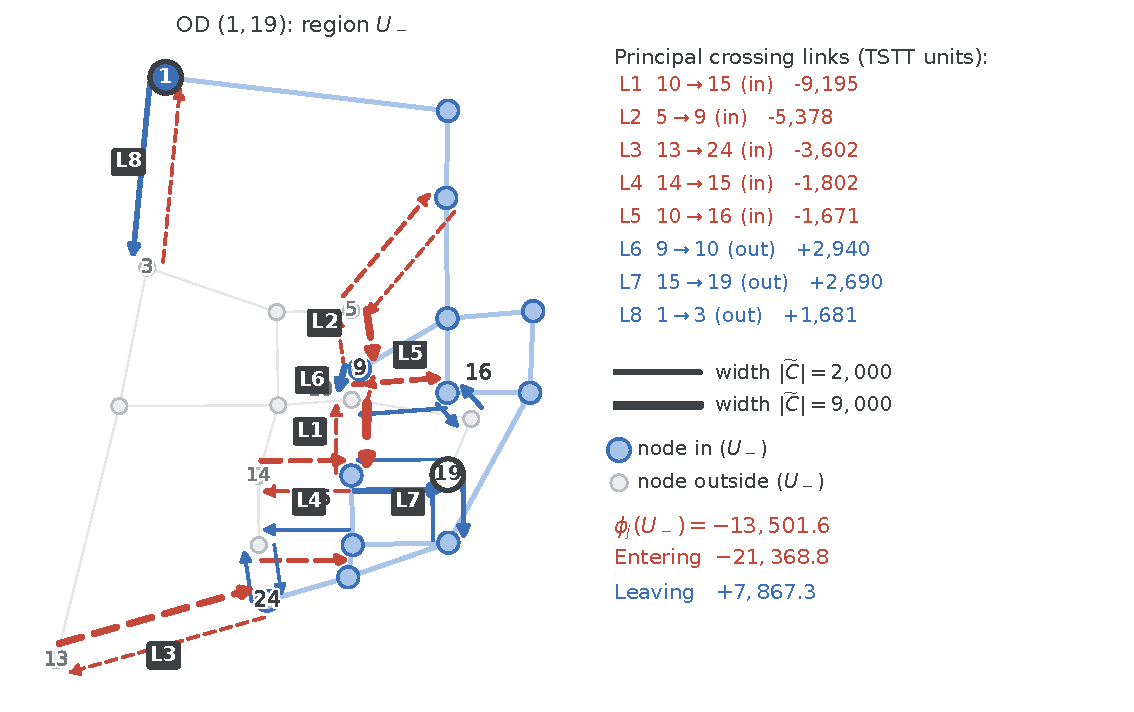
\includegraphics[width=0.82\linewidth]{../figures/fig_negmech_v102.pdf}
\caption{The connected minimizing region $U_-$ for OD $(1,19)$
(responsive-background six-query protocol). Shaded nodes form $U_-$ (origin
node $1$ ringed; destination $19$ outside). Crossing-link arrows keep
the link direction; width scales with $|\widetilde C_{e,j}|$, and
colour and style encode the signed contribution to $\phi_j(U_-)$,
$a_{e,j}=\sigma_e\widetilde C_{e,j}$ ($\sigma_e=+1$ leaving, $-1$
entering; solid blue positive, dashed red negative), so a positive
attribution on an entering link appears red. The side panel lists, in
TSTT units, the five largest negative and three largest positive
contributions among the $26$ crossing links
($\mathrm{L}1$--$\mathrm{L}5$ negative, $\mathrm{L}6$--$\mathrm{L}8$
positive, ``(in)''/``(out)'' marking entering and leaving links),
with the width scale and the membership legend.}
\label{fig:negmech}
\end{figure}

\FloatBarrier
\subsection{Frozen-surrogate boundary errors}\label{supp:screenlinelearned}
On the six-query connected families, the five frozen flow-supervised
surrogates of the earlier protocol show five-seed median
largest-boundary disagreements of $4.2$--$6.9\%$ of the direct
connected span for four queries, rising to $99.5\%$ for the
small-response query $(4,5)$ and beyond the span for $(7,18)$ --- a
further early indicator that flow-only supervision does not control
boundary error. Sign reliability, by contrast, is boundary specific:
all five seeds retain the three connected-family sign crossings and
positive system contributions, and at the fixed direct-model minimizing
screenline every seed keeps the negative sign for $(1,19)$ and
$(7,12)$ (seed ranges $[-3886.6,-3365.1]$ and $[-2810.4,-1916.6]$
against references $-2766.6$ and $-2967.3$, with largest family-wide
errors below the reference sign margins). These are screenline-specific
certificates of sign preservation, not of column magnitudes; the
per-query screenline table and across-seed envelopes accompany the
result arrays.

\subsection{Numerical diagnosis of the transferability hierarchy}\label{supp:levelsdiag}
The universal structural condition quantifies over all conservative
responses; Section~\ref{sec:levels} introduced the model-specific level
that reasons on the path-feasible response envelope of the assignment
model's fixed path sets.
Table~\ref{tab:levelsdiag} evaluates the hierarchy numerically. On the
Figure-1 network with its published post-merge weights, the universal
condition fails because the off-path pendant atom is heterogeneous, yet
the model-specific tests hold exactly for the all-simple-paths
structure: every rerouting that model can make preserves the common
account, so restricting attention to the path-feasible envelope
restores transferability that the universal condition denies. On Sioux
Falls the two levels coincide --- the full-background fixed-path model
spans the complete circulation space through path exchanges, so its
path-feasible envelope contains every conservative response
(Appendix~\ref{supp:networks}) --- and both fail at realistic TSTT
weights, leaving the realized summaries of Table~\ref{tab:newod} as the
operative output. The diagnosis is stable across load levels: the
normalized universal violation stays within $2.08$--$2.21$ from the
$0.7$ to the $1.3$ baseline while $\rho_{\mathrm{swap}}$ falls from
$1.12$ to $0.80$ as congestion grows. On Anaheim the universal test
fails more decisively (normalized violation $10.08$) and the
model-specific test fails with it ($\rho_{\mathrm{swap}}=2.18$ over the
$404$-dimensional exchange space), so there too the realized layer
carries the reporting.

\begin{table}[t]\centering\footnotesize
\caption{Numerical diagnosis of the transferability hierarchy of
Table~\ref{tab:threequestions}. $\eta_{\mathrm{all}}$ and
$\eta_{\mathrm{conn}}$: weight spread within all atoms / within the
queried atoms, normalized by the mean weight. $\rho_{\mathrm{swap}}$:
weighted-divergence leakage of unit rerouting directions relative to a
unit reference response; $\rho_{\mathrm{swap}}=0$ certifies
$BDN=0$, and together with zero off-span residuals
$\rho_{\mathrm{ref},j}$ it certifies both conditions of the
model-specific level. On Sioux Falls (level $1.0$) three of the six
queries have $\rho_{\mathrm{ref},j}=0$; the other three lie in
$0.83$--$0.97$. Realized: median
normalized geometric common-summary error of the responsive-background six
queries. Synthetic: published post-merge weights; Sioux Falls: TSTT
weights at the level-$1.0$ equilibrium, where the path-exchange space
attains the full circulation dimension $53$.}\label{tab:levelsdiag}
\begin{tabular}{lrrrr}\toprule
Network & $\eta_{\mathrm{all}}$ & $\eta_{\mathrm{conn}}$ & $\rho_{\mathrm{swap}}$ & Realized (\%)\\\midrule
Figure-1 synthetic & $0.61$ & $0$ & $0$ & $0$ (model responses)\\
Sioux Falls & $2.08$ & $=$ & $0.88$ & $32.3$\\
\bottomrule\end{tabular}\end{table}

\subsection{Additional learning comparisons}\label{app:legacy-learning}\label{app:learning-protocol}\label{app:calibration-protocol}
The attribution-column error of a learned model splits exactly into a
weight-shift and a response term ($L$/$S$: learned/direct in
Eq.~\eqref{eq:Cdef}):
\begin{equation}
\widetilde C_{:,j}^{L}-\widetilde C_{:,j}^{S}
=\Delta q_j\int_0^1(D_\lambda^{L}-D_\lambda^{S})J_j^{S}\,\mathrm{d}\lambda
+\Delta q_j\int_0^1D_\lambda^{L}(J_j^{L}-J_j^{S})\,\mathrm{d}\lambda,
\label{eq:coldecomp}
\end{equation}
satisfied entrywise within $10^{-10}$ TSTT units on the 96 test paths;
the weight-shift term has querywise median norm at most 0.2\% of the
reference column and the response term is larger in every seed--query
unit.

Two earlier pointwise comparisons test fixed-coefficient boundary
supervision and validation-calibrated coefficients against response
supervision, from the same five conservative models with 600 Adam
updates at $3\times10^{-5}$ and batches 32/8 (derivative labels: 256
training and 64 validation states; four prescribed 41-state test paths
with one, two, three and six active queries). Fixed-coefficient
supervision yields 22.25\% boundary error versus 9.64\% for response
supervision; calibration yields 7.74\% versus 7.44\%. Neither
comparison supports overall improvement. The final six-objective
comparison with common selection and matched-path metrics is
Table~\ref{tab:fairmethods}.

\subsection{Group-level uncertainty for the 96-path comparison}\label{supp:learningdetail}
\begin{table}[pos=htbp]\centering\footnotesize
\caption{Per-seed medians of path-level values on the 96 paths and
path-level improvement counts (response vs.\ flow supervision).}\label{tab:fiveseed}
\setlength{\tabcolsep}{4.5pt}
\begin{tabular*}{\tblwidth}{@{\extracolsep{\fill}}r cc cc cc}
\toprule
& \multicolumn{2}{c}{Column (\%)} & \multicolumn{2}{c}{Geometric (\%)} & \multicolumn{2}{c}{Improved paths}\\
\cmidrule(lr){2-3}\cmidrule(lr){4-5}\cmidrule(lr){6-7}
Seed & flow & resp. & flow & resp. & col. & geo.\\
\midrule
0 & 19.55 & 15.93 & 8.40 & 5.67 & 85/96 & 84/96\\
1 & 15.66 & 12.44 & 7.07 & 4.57 & 80/96 & 84/96\\
2 & 22.81 & 14.91 & 9.08 & 6.52 & 88/96 & 89/96\\
3 & 22.33 & 14.95 & 7.40 & 5.98 & 87/96 & 84/96\\
4 & 16.65 & 12.02 & 6.57 & 4.23 & 87/96 & 91/96\\
\bottomrule\end{tabular*}\end{table}

Path-level bootstrap intervals for the paired median differences
(10,000 resamples; column error / family-boundary error, in percentage
points): single-query group $[-4.90,-2.95]$ / $[-1.99,-0.88]$
improving 24/24 and 23/24 paths; two-query group $[-6.48,-4.31]$ /
$[-3.15,-1.52]$, 22/24 and 21/24; three-query group $[-9.26,-3.36]$ /
$[-4.11,-1.36]$, 22/24 and 22/24; six-query group $[-8.59,-5.22]$ /
$[-3.86,-1.73]$, 24/24 and 24/24. Leave-one-path-out medians of the
paired column difference vary within $[-5.11,-4.94]$ and of the paired
family-boundary difference within $[-2.11,-2.00]$, so no single path
carries the result. The system-contribution difference has median
$+0.45$ percentage points with interval $[0.01,0.74]$, improving 39 of
96 paths, while both methods retain system errors below $3.5\%$
(medians $2.52\%$ and $3.13\%$).

The incremental-flow error of the main text (per path--seed medians;
reference increments are well conditioned --- smallest reference
increment norm $45$ veh/h on Sioux Falls and $508$ veh/h on Anaheim
against medians of $258$ and $1{,}672$): on Sioux Falls
$5.14\%$ under flow supervision and $3.46\%$ under response
supervision (absolute numerators $13.6$ and $8.8$ veh/h); on Anaheim
$2.46\%$ and $2.08\%$ ($38.6$ and $33.2$). Response supervision
therefore improves not only the boundary attributions but also the
incremental flow response from which they are integrated, while the
total-flow errors of Table~\ref{tab:pathtable} stay near $0.03\%$
because total flows are dominated by the unchanged background.

\subsection{Unrestricted and integrated-bound errors by group}\label{supp:boundchain}
Table~\ref{tab:boundchain96} completes Table~\ref{tab:pathtable} with
the unrestricted and integrated-bound columns of
Eq.~\eqref{eq:localboundarybound}, as percentages of the reference
column's boundary seminorm; the geometric and unrestricted columns use
different denominators and are not one inequality, and the bound chain
$\mathcal K_j(e_j)\le B_j$ holds in absolute units for the shared
quadrature (Section~\ref{sec:pairresults}).
\begin{table}[pos=htbp]\centering\footnotesize
\caption{Unrestricted (exact $\mathcal K_j(e_j)$ over all separating
regions) and bound (integrated bound of
Eq.~\eqref{eq:localboundarybound}) errors, medians of path-level values
on the 96 test paths, as percentages of the reference column's
boundary seminorm.}\label{tab:boundchain96}
\begin{tabular}{rcc cc}\toprule
& \multicolumn{2}{c}{Unrestricted (\%)} & \multicolumn{2}{c}{Bound (\%)}\\
\cmidrule(lr){2-3}\cmidrule(lr){4-5}
Active & flow & resp. & flow & resp.\\\midrule
1 & 4.54 & 2.95 & 4.62 & 3.00\\
2 & 15.48 & 12.65 & 15.67 & 12.80\\
3 & 16.36 & 12.39 & 16.70 & 12.81\\
6 & 19.43 & 12.28 & 20.61 & 13.48\\
\midrule
All 96 & 15.65 & 12.08 & 16.34 & 12.83\\
\bottomrule\end{tabular}\end{table}

\subsection{Complete input-stratified common-summary results}\label{sec:coverage}
Positive non-diagonal published demands are stratified by demand and directed free-flow shortest-path time using empirical tertiles, with ties kept in the lower bin. Within each of nine cells, lexicographically sorted OD indices at zero-based positions $\lfloor N/3\rfloor$ and $\lfloor2N/3\rfloor$ are retained. No attribution values enter selection. Endpoint differences identify total edge attribution, without identifying the same-state study/background response split. The two perturbation widths share every field of the selection protocol and differ only in the demand interval; their normalized errors are close for every query, so Table~\ref{tab:coveragefull} reports both in one table. Each query's common value and error follow from the tabulated range by the midpoint rule $\beta=(\phi_{\min}+\phi_{\max})/2$; absolute minima, maxima, midpoints and half-ranges for both widths, the complete normalized interval set, and the per-position account sequences behind the segmentation of Proposition~\ref{prop:segmented} accompany the result arrays in the code package.
\begin{table}[pos=htbp]\centering\footnotesize\caption{Complete geometric common summaries for the 18 input-stratified queries at both widths. Normalized error is Eq.~\eqref{eq:normerror} at $\pm10\%$ and $\pm20\%$; ranges are $[\phi_{\min},\phi_{\max}]$ at $\pm20\%$ in Sioux Falls cost units; P and M mean positive and mixed signs at $\pm20\%$.}\label{tab:coveragefull}\begin{tabular}{lrrrrl}\toprule OD & System & Range ($\pm20\%$) & Norm.\ err.\ ($\pm10\%$) & Norm.\ err.\ ($\pm20\%$) & Sign\\\midrule
(4,3) & 507.2 & [429.0, 535.0] & 9.9 & 9.9 & P\\
(12,3) & 337.2 & [330.7, 340.2] & 1.4 & 1.4 & P\\
(6,1) & 2360.6 & [658.3, 2290.4] & 35.6 & 35.6 & P\\
(15,6) & 9390.2 & [415.4, 4433.5] & 45.3 & 45.3 & P\\
(6,21) & 4577.8 & [-3.4, 2349.4] & 50.1 & 50.1 & M\\
(18,14) & 3422.3 & [150.8, 1929.7] & 46.1 & 46.1 & P\\
(8,4) & 25097.5 & [1270.7, 15741.3] & 46.0 & 46.0 & P\\
(19,8) & 16939.7 & [733.2, 7266.4] & 45.0 & 45.0 & P\\
(11,6) & 6165.9 & [1236.4, 6106.4] & 39.9 & 39.9 & P\\
(16,2) & 17763.1 & [896.3, 9628.6] & 45.3 & 45.3 & P\\
(8,21) & 7605.5 & [752.6, 4214.1] & 41.1 & 41.1 & P\\
(14,8) & 17445.3 & [890.3, 7527.1] & 44.1 & 44.1 & P\\
(11,15) & 47925.5 & [17628.9, 27737.8] & 18.2 & 18.2 & P\\
(17,9) & 24040.9 & [5482.3, 18519.3] & 35.2 & 35.2 & P\\
(10,12) & 55214.5 & [9822.4, 33248.6] & 35.2 & 35.2 & P\\
(13,10) & 54411.9 & [2918.8, 31345.2] & 45.3 & 45.3 & P\\
(1,10) & 33917.2 & [2182.9, 20856.4] & 44.8 & 44.8 & P\\
(10,1) & 34264.5 & [2182.7, 21039.5] & 44.8 & 44.8 & P\\
\bottomrule\end{tabular}\end{table}

\begin{table}[pos=htbp]\centering\footnotesize
\caption{Tolerance sensitivity of the delivered summaries, within
fixed projection directions (the input-stratified selection experiment for Sioux Falls, 18 queries
per level, 36 normals with duplicate chains removed; the Anaheim ordered-family experiment for
Anaheim, six single-direction queries). Single: number of queries whose
whole family admits one common value at the stated tolerance;
segments: median per-direction count on Sioux Falls at load levels
$0.7/1.0/1.3$ (maximum over directions in parentheses) or per-query
range on Anaheim; compression: $1-$segments/regions, median per
direction (Sioux Falls) or per query (Anaheim).}\label{tab:tolerance}
\begin{tabular}{rrrrr}\toprule
Tolerance $\tau$ & Sioux single ($0.7/1.0/1.3$) & Sioux med.\ seg./dir. & Anaheim segments & Anaheim compression\\\midrule
$2.5\%$ & $2/1/0$ & $4.0\,(10)/4.5\,(12)/5.5\,(13)$ & $6$--$21$ & $91.5\%$\\
$5\%$ & $2/1/0$ & $3.0\,(7)/4.0\,(8)/4.5\,(10)$ & $4$--$14$ & $93.8\%$\\
$7.5\%$ & $2/1/1$ & $2.0\,(7)/3.0\,(8)/3.0\,(8)$ & $3$--$12$ & $95.5\%$\\
$10\%$ & $2/2/1$ & $2.0\,(6)/2.0\,(6)/2.5\,(7)$ & $3$--$12$ & $96.4\%$\\
\bottomrule\end{tabular}\end{table}

\paragraph{Tolerance rule and small-magnitude detail.}\label{supp:tolerance}
The primary rule is absolute: $\epsilon_j=5\%$ of the family's largest
account magnitude, so it permits errors much larger than $5\%$ of the
small accounts. A mixed rule
$|\hat a_i-a_i|\le\epsilon_{\mathrm{abs}}+\tau|a_i|$ keeps relative
control at small magnitudes; a candidate segment admits a common
representative iff $\max_{i\in I}(a_i-t_i)\le\min_{i\in I}(a_i+t_i)$
with $t_i=\epsilon_{\mathrm{abs}}+\tau|a_i|$, feasibility is inherited
by subintervals, and the same greedy returns the minimum count. On
Anaheim, at the primary rule the worst relative error at
small-magnitude positions (accounts below $10\%$ of the family
maximum) has median $0.55$ and maximum $0.94$; the mixed rule with
$\epsilon_{\mathrm{abs}}=1\%$ of the family maximum and $\tau=10\%$
lowers these to $0.28$ and $0.45$ while the median segment count rises
from 10 to 12 (per-query range 6--17), i.e.\ the compression is
essentially retained and the detail at small-magnitude positions
doubles in accuracy. Enlarging the relative part of the primary
$5\%$ absolute rule without shrinking the absolute floor
($\epsilon_{\mathrm{abs}}=5\%$, $\tau\ge5\%$) instead reduces
segment counts by merging large-magnitude runs while the
small-position error worsens --- confirming that the absolute floor,
not the relative part, controls the small-magnitude detail.

\paragraph{Load-level protocol and node-imbalance diagnostics.}
The load-level experiment solves one equilibrium per level ($0.7$,
$1.0$, $1.3$ times the published demands), the focal query moving
alone over $\pm20\%$ under the identical geometric family. Across the
54 query--level pairs, the node-imbalance norm $\norm{d_j}_2$ of
Eq.~\eqref{eq:endpointd} rises $13.2$-fold from the light to the
heavy baseline (medians $1196.4$ to $15763.3$), tracks the
geometric-family spread and the unrestricted range $S_j$ with rank
correlation $0.99$, and the realized ratio $S_j/\norm{d_j}_2$ has
median $2.53$ against the Cauchy--Schwarz bound $\sqrt{n-2}=4.69$ of
Eq.~\eqref{eq:cutgap} --- mechanism-consistent readings of
Eq.~\eqref{eq:cutspread} in which the load levels change realized
weights, responses and demand increments together.

\subsection{Computational protocol for alternative attribution orders}\label{supp:pathrobust}
Each of the 22 alternative orders of Section~\ref{subsec:pathrobust}
changes the six study ODs one at a time (41 quadrature states per
segment, identical solver tolerance, endpoints and boundary family as
the straight-line run; canonical order, reverse order, and twenty
permutations under seed 20261031). Gates: straight-line columns
reproduce the frozen arrays to $1.7\times10^{-15}$ relative; every
order's endpoint equilibria match the straight-line endpoints to
$6.1\times10^{-9}$; the path-independent total outcome change
reproduces to $1.5\times10^{-7}$ relative. Each order's record stores
the attribution column, family range, common summary and normalized
error, sign-crossing flag, maximum profile deviation against the
straight-line accounts, and mechanism components at the fixed regions
$U_-$ (arrays in the code package). The dominant mechanism at $U_-$
coincides with the straight line's on all 22 orders for each of the
three mechanism-tracked queries.

\begin{table}[t]\centering\footnotesize
\caption{Attribution-path robustness on the responsive-background six-query
protocol: straight-line joint path versus 22 one-at-a-time orders
(canonical, reverse, 20 seeded permutations). $C_j$ range: minimum and
maximum over the orders; deviation relative to the straight-line
value. $\varepsilon$ shift: median normalized common-summary error
over the orders against the straight-line value. Sign: orders whose
family range keeps the straight-line sign-crossing status; mechanism:
orders whose largest-magnitude component at $U_-$ matches the straight
line's.}\label{tab:pathrobust}
\begin{tabular}{lrrrrr}\toprule
OD & $C_j$ range & Max $|C_j|$ dev. & $\varepsilon$ shift & Sign & Mechanism\\\midrule
$(7,18)$ & $[666.5,\ 678.4]$ & $1.0\%$ & $4.3\%\to4.3\%$ & $22/22$ & ---\\
$(1,19)$ & $[48{,}451.9,\ 51{,}817.7]$ & $3.4\%$ & $56.3\%\to56.4\%$ & $22/22$ & $22/22$\\
$(4,5)$ & $[2{,}780.8,\ 2{,}911.4]$ & $3.0\%$ & $8.2\%\to8.2\%$ & $22/22$ & ---\\
$(1,15)$ & $[75{,}306.6,\ 79{,}553.2]$ & $2.8\%$ & $49.3\%\to49.3\%$ & $22/22$ & $22/22$\\
$(6,8)$ & $[72{,}157.8,\ 75{,}713.7]$ & $2.4\%$ & $15.4\%\to15.5\%$ & $22/22$ & ---\\
$(7,12)$ & $[117{,}367.2,\ 117{,}573.5]$ & $0.1\%$ & $52.6\%\to52.5\%$ & $22/22$ & $22/22$\\
\bottomrule\end{tabular}\end{table}

\subsection{Anaheim learned-assignment protocol}\label{app:anaheimlearning}
The Anaheim experiment mirrors the Sioux Falls protocol in structure;
differences are stated here once. The study queries are the six largest
published OD demands of Section~\ref{sec:anaheim}; all remaining
positive demands are fixed with endogenous route choice over the same
ten-path centroid-restricted structure. The model is the conservative
parameterization of Eq.~\eqref{eq:consparam} with $K=1{,}406$ OD
softmaxes over $P=14{,}060$ paths and $m=914$ link outputs; the input
is the six-dimensional study demand vector. Reference labels: 1{,}000
flow states ($q\sim U(0.65,1.3)\,q_{\mathrm{base}}$; 800 train, 200
validation), 480 derivative centers (384 train, 96 validation) with
equilibrium sensitivities of the six study columns, and 48 test demand
paths (twelve per active-query group $k\in\{1,2,3,6\}$, mixed and same
signs, generation rule identical to the Sioux Falls test paths under a
fresh seed) solved at a 21-state quadrature with sensitivities at every
state. Training: stage~A pretrains flow-only from scratch for up to
4{,}000 steps (Adam, learning rate $3\times10^{-3}$, batch 128,
per-link scaled MSE, best-validation selection every 50 steps); stage~B
continues for 1{,}200 steps with the method objective exactly as in
the Sioux Falls protocol (learning rate $3\times10^{-5}$, batch 32
flow samples plus 8 derivative centers, rotation over the six study
columns), methods \emph{flow} and \emph{response}, five seeds.
Validation: flow relative error on the 200 held-out flow states;
$K$-MSE, the boundary-seminorm of the weighted response discrepancy
normalized per query, on the 96 held-out centers. Selection: minimum
validation $K$-MSE among states with validation flow error at most
1.1 times the stage-A checkpoint, fallback minimum flow error; test
paths enter neither training nor selection. Selected checkpoints
cluster at the training cap, as in Sioux Falls, so the operating
point is budget-limited rather than validation-plateaued; the
extended-budget replication below triples the cap under the identical
rule. Gates: conservation of every reference state (study plus
background supply) holds to $9.1\times10^{-12}$ vehicle-units;
reference-column completeness relative to the endpoint outcome change
is at most $1.2\times10^{-5}$; the total error of every delivered
summary stays within its budget. Costs: reference data 2{,}488
equilibrium solves with sensitivities ($\approx$35\,s per state
single-threaded, parallelized over twelve workers), pretraining
$\approx$40\,minutes per seed, fine-tuning $\approx$5--9\,minutes per
(method, seed).

\paragraph{Extended budget.}
The convergence check of Section~\ref{sec:pairresults} repeats the
stage-B continuation for both methods and five seeds with the budget
tripled to 3{,}600 updates: identical initialization, learning rate,
batches, label sets, validation cadence and selection rule, and the
same test paths for the final report. On Sioux Falls the replication
asserts that the first twelve validation points (the original
1{,}200-update budget) reproduce the archived runs to $10^{-12}$ in
validation boundary error, so the extension is an exact continuation
of the frozen protocol. Every Anaheim run selects beyond the original
cap (all five response seeds at 3{,}600 updates); the archived
3{,}600-update fine-tuning takes $\approx$30--105 minutes per
(method, seed) single-threaded on Anaheim and $\approx$4--6 minutes
per run on Sioux Falls.

